\chapter{Системийн архитектур, зохиомж}

\section{Системийн архитектур}

Манай систем нь тийм ч төвөгтэй систем биш мөн энгийн веб хөтчүүдэд зориулж хийгдэх тул системийн архитектурын үлгэр загвар дундаас веб аппд хамгийн өргөн хэрэглэгддэг Хэрэглэгч-Сервер (Client-Server pattern) үлгэр загварыг сонголоо. Хэрэгжүүлэхэд хялбараас гадна Next.js, Prisma ашиглан төслөө хөгжүүлж байгаа учир хамгийн тохиромжтой гэж үзэж байна.

\begin{figure}[h]
	\centering
	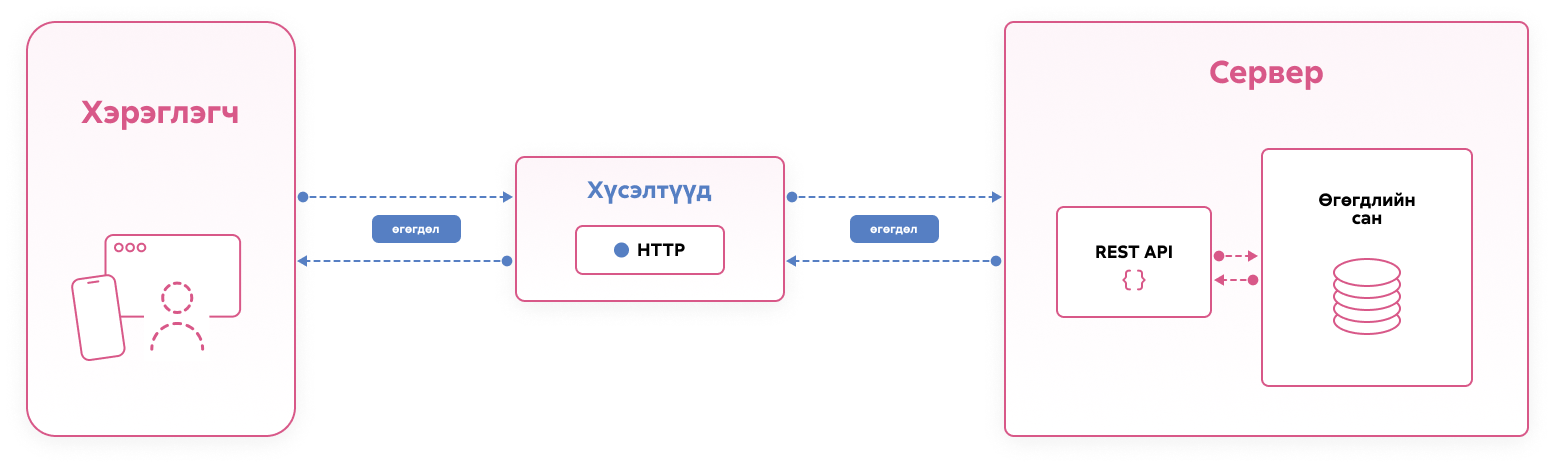
\includegraphics[width=15cm]{images/architecture.png}
	\caption{Client-Server Архитектурын үлгэр загварын дүрслэл}
	\label{fig:architecture}
\end{figure}

Хэрэглэгч талаас компьютер, гар утасны веб хөтчийг ашиглаж HTTP холболтоор хүсэлт явуулж, сервер талаас өгөгдлийн санг ашиглан REST API бэлдэн эргээд хэрэглэгч рүү HTTP холболтоор хүсэлтийн хариуг өгөх зарчмаар ажиллана.

\section{Ажлын явцын диаграм}

\begin{figure}[h]
	\centering
	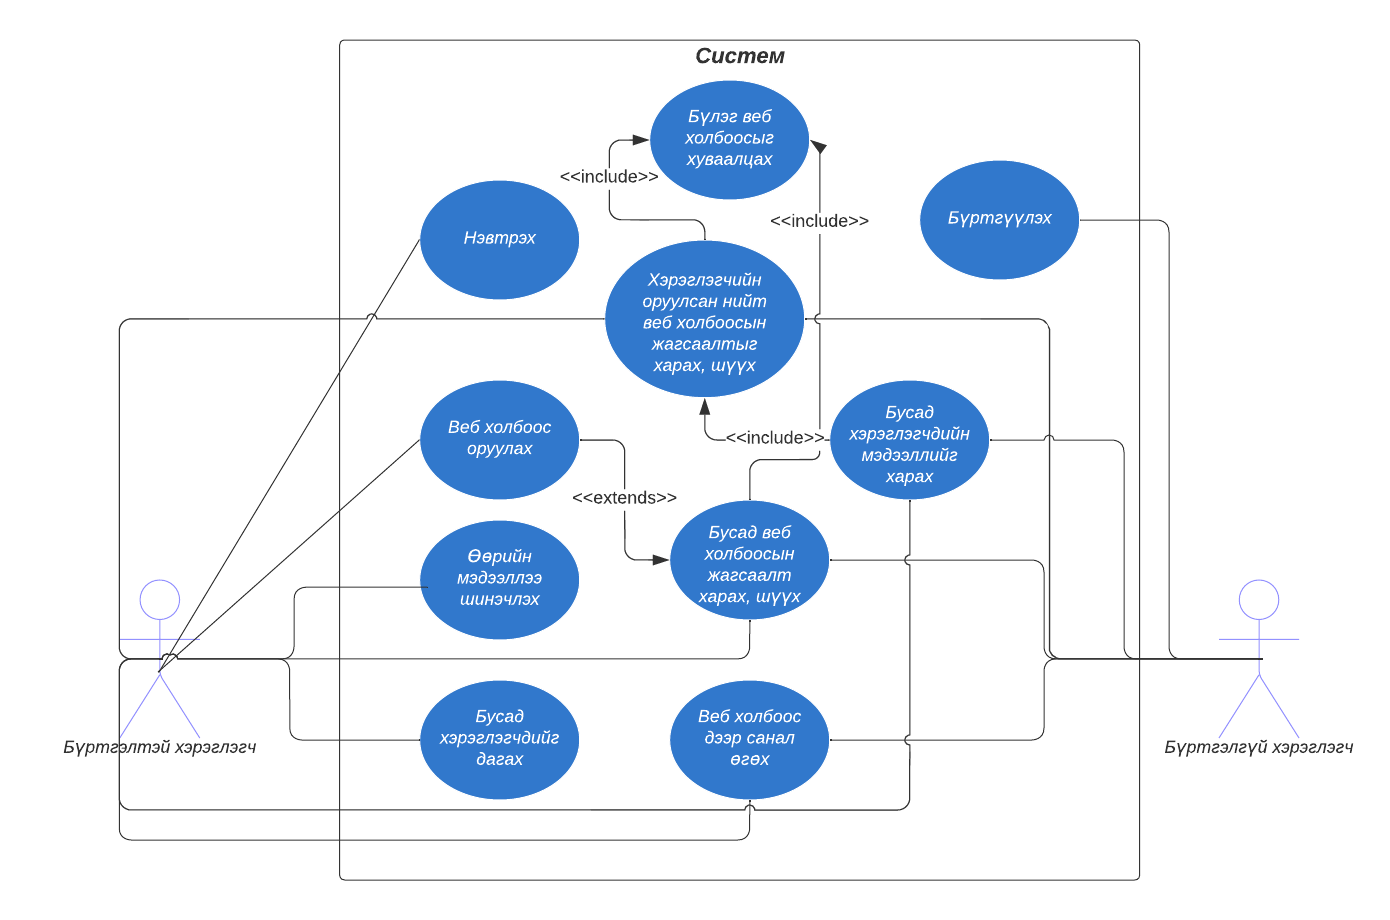
\includegraphics[width=15cm]{images/usecase.png}
	\caption{Ажлын явцын диаграм}
	\label{fig:usecase}
\end{figure}

\pagebreak
\textbf{Ажлын явцын диаграмын тайлбар}

\begin{itemize}
	\item \textbf{Нэвтрэх -} Бүртгэлтэй хэрэглэгч өөрийн бүртгүүлсэн имэйл хаягаараа нэвтрэх, нууц үгээ сэргээх
	\item \textbf{Веб холбоос оруулах -} Өөрийн хүссэн веб холбоосоо дангаар нь болон бүлэглэж оруулах, хэрэв бүлэглэж оруулахаар бол тухайн бүлэг веб холбоосны нэр, тайлбаруудыг заавал авна
	\item \textbf{Өөрийн мэдээллээ шинэчлэх -} Өмнөх мэдээлэл хуучирсан эсвэл шинэчлэх шаардлага гарсан тохиолдолд хувийн мэдээлэл, холбооснуудынхаа нууцлалыг шинэчлэх
	\item \textbf{Бусад хэрэглэгчдийг дагах -} Өөрийн нүүр хуудсаа сонирхлынхоо дагуу хөгжүүлэхийг хүсвэл бусад хэрэглэгчдийг дагаж, тэдгээрийн оруулсан холбооснуудыг хамгийн эхэнд харах
	\item \textbf{Бусад веб холбоосын жагсаалтыг харах -} Систем дээр public байдлаар нийтлэгдсэн бүх веб холбоосыг шууд болон шүүсэн байдлаар харж өөрт хэрэгтэй мэдээллээ авах
	\item \textbf{Веб холбоос дээр санал өгөх -} Бүртгэлтэй болон бүртгэлгүй хэрэглэгчид тухайн веб холбоосны контентыг харсны дараагаар өөрийн хувийн саналаа өгч, чанарын үнэлгээ хийх 
	\item \textbf{Бүртгүүлэх -} Хэрэглэгч бүртгэлгүй хэдий ч манай платформыг бүрэн ашиглах боломжтой. Хэрэв өөрөө веб холбоос оруулахыг хүсвэл хувийн мэдээллээ бөглөж бүртгүүлэх
	\item \textbf{Хэрэглэгчийн оруулсан нийт веб холбоосын жагсаалтыг харах -} Зөвхөн нэг хэрэглэгчийн оруулсан private болон public веб холбооснуудыг нэг хуудсан харах, тэдгээрээс шүүх
	\item \textbf{Бусад хэрэглэгчдийн мэдээллийг харах -} Бүртгэлтэй болон бүртгэлгүй хэрэглэгч бусад хэрэглэгчдийн оруулсан хувийн мэдээллийг харах, холбоо барих мэдээллийг олох
	\item \textbf{Бүлэг веб холбоосыг хуваалцах -} Хэрэглэгч нэг сэдвийн хүрээнд олон веб холбоос оруулсан бол платформ дээр тухайн бүлгийн мэдээллийг харуулсан тусдаа нэг хуудас үүснэ. Түүний веб холбоосыг хуулж авах, бусад сошиал сүлжээнд түгээх
\end{itemize}

\section{Өгөгдлийн сангийн диаграм}
\section{Дарааллын диаграм}
\section{Хэрэглэгчийн интерфейс дизайн}

